\subsection{Parallel Execution}\label{section: parallel-execution}

\subsubsection{Challenges in Parallel Transaction Execution}

The transaction execution process for most blockchains is as follows: the execution module sequentially retrieves transactions from the block and executes them one by one. During execution, the latest world state is modified. When a transaction is completed, the state is accumulated until the latest world state is reached after the completion of the block. The execution of the next block strictly depends on the world state after the execution of the previous block. Therefore, it is difficult to optimize parallel execution in the traditional linear transaction execution process.

In traditional blockchain projects, transactions cannot be directly executed in parallel, mainly due to the following types of race conditions:

\begin{enumerate}
    \item Account conflicts: If two threads process the balance or other attributes of the same address account simultaneously, the result must be consistent with sequential processing, meaning the world state is a deterministic finite state machine.
    \item Same-address storage conflicts: Two contract variables modify the storage of the same global variable simultaneously.
    \item Cross-contract call conflicts: Contract A must be deployed first, and Contract B calls Contract A after Contract A is deployed. However, after parallel transaction execution, the order no longer exists, leading to conflicts.
\end{enumerate}

\subsubsection{OlaVM Parallel Transaction Execution Solution}

The implementation of OlaVM is as follows: each transaction within the same block starts from the world state of the previous block and is executed in parallel. During execution, all three types of race conditions encountered in the ideal execution path are recorded. After the parallel execution phase is finished, the merge phase begins. The merge phase sequentially combines the world state. When merging each transaction, First, determine if there is a conflict.  If there are no conflicts, merge directly; if conflicts exist, re-execute the transaction from the starting point of the merged world state to obtain a new world state.

If the current node needs to process blocks synchronized from other nodes, the processing flow is as follows:

\begin{enumerate}
    \item The node starts the parallel transaction execution process.
    \item After the parallel transaction execution is completed, the node merges the world state.
    \item The node verifies the final merged world state using the synchronized block hash.
    \item If the verification is correct, the node broadcasts the block to the network.
    \item If the verification is incorrect, the node re-executes the block sequentially.
\end{enumerate}

In general, if the computing task can be fully parallelized, the scalability of a single chain will be enormous. This is because nodes can add more CPU cores. However, the actual situation is not like this. The maximum theoretical speed is limited by Amdahl's Law\cite{website:Amdahls-law}: the speedup limit of the system depends on the reciprocal of the non-parallelizable part. For example, if 99\% parallelism can be achieved, the speed can be increased 100 times; if only 95\% parallelism can be achieved, the speed can be increased 20 times.

For the replay of all Ethereum transactions, about 80\% of transactions can be parallelized, while the remaining 20\% cannot be parallelized. Therefore, the theoretical speed-up limit of Ethereum transaction processing using this solution is about 5 times.

For block producers, since they can be deployed on higher-performance machines, If they can accurately identify the conflicting conditions of different transactions and sort these transactions according to the best strategy, the parallelism may be greatly improved, thus achieving higher speedup.

The transaction process is executed in parallel as shown in the figure:\ref{fig:paralle-execution}

\begin{figure}[!ht]
    \centering
    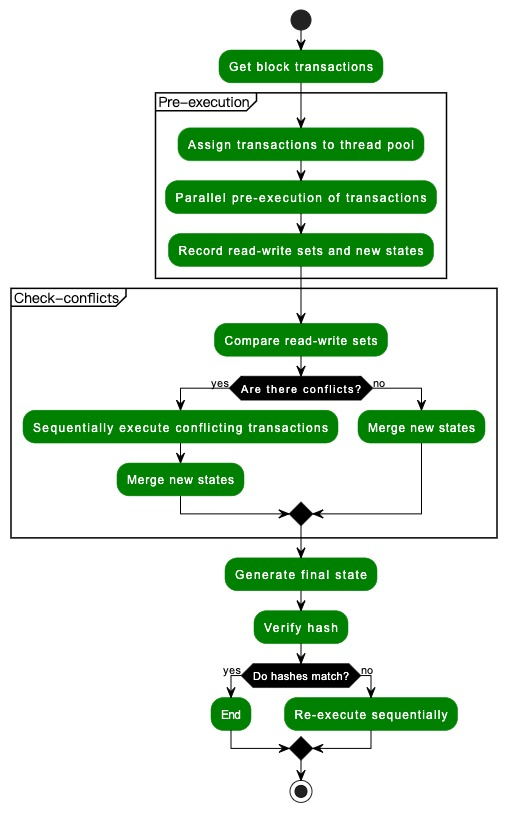
\includegraphics[width=0.6\textwidth]{images/paralle-execution.jpg}
    \caption{Parallel Transaction Execution Process}
    \label{fig:paralle-execution}
\end{figure}

\subsubsection{Conflict Transaction Marking}

In EVM, conflicts mainly occur during the process when certain instructions perform read and write operations on storage. By recording these read-and-write operations, a read-and-write set can be formed. However, static code analysis cannot ensure that all these processes are recorded. Therefore, when processing transactions in each block, each transaction needs to be pre-executed in parallel. Through the pre-execution process, it can be understood whether these transactions perform read and write operations on the same account or storage, and then a read-set and write-set can be generated for each transaction. The pre-execution process first copies the world state multiple times as the initial state for all transactions. Suppose there are 100 transactions in the blockchain; these 100 transactions can be executed in parallel through a thread pool. Each contract has the same initial world state, and during execution, 100 read-sets and write-sets will be generated, along with 100 new states.

After the pre-execution is finished, the next phase begins. Ideally, if these 100 read-sets and write-sets have no conflicts, they can be directly merged to produce the final world state after all transactions in the block have been executed. However, conflicts in merger transactions usually do not proceed smoothly. The correct way is to first compare the read-sets and write-sets after the execution of the first and second transactions to see if they perform read and write operations on the same account or storage. If there is a conflict, it means that these two transactions have conflicts. At this point, the state after the completion of the first transaction will be used as the starting state for the second transaction, and the second transaction will be re-executed. In this way, as the state machines are continuously merged, the conflict set will continue to accumulate. As long as subsequent transactions have conflicts with previous transactions, they will be executed sequentially until all transactions are completed.

\subsubsection{Advantages and Disadvantages of the Solution}

Advantages: Improved parallel speed, and enhanced security without using locks. Since the state merging itself is not the focus of time consumption, it basically won't form a bottleneck.

Disadvantages: Putting all transaction validations at the end of the processing phase may lead to performance degradation when there are many transaction conflicts. However, for Ethereum transactions, there are relatively few conflicting items, so the performance is expected to increase by about 3 to 5 times.
